% The step mapping theta [FIPS 202, §3.2.1, Figure 3]: each bit is XORed with the parities of
% column x - 1 in its own slice and of column x + 1 in the previous slice z - 1.
% Original drawing for the Hash library.
\documentclass[tikz,border=6pt]{standalone}
\usepackage[T1]{fontenc}
\usepackage{lmodern}
% Shared style for the Hash diagrams.
% Palette: Okabe–Ito (colour-blind safe). Every diagram is drawn on an opaque white card so it
% stays legible on dark page themes.
\usetikzlibrary{arrows.meta,positioning,calc,fit,backgrounds}
\definecolor{hsblue}{HTML}{0072B2}
\definecolor{hsorange}{HTML}{E69F00}
\definecolor{hsgreen}{HTML}{009E73}
\definecolor{hsvermilion}{HTML}{D55E00}
\definecolor{hspurple}{HTML}{CC79A7}
\definecolor{hsink}{HTML}{1F2933}
\tikzset{
  >={Stealth[length=2.2mm]},
  every node/.style={font=\sffamily\small, text=hsink},
  wire/.style={draw=hsink, line width=0.6pt, ->},
  reg/.style={draw=hsink, line width=0.6pt, fill=hsblue!12, minimum width=9mm, minimum height=7mm},
  fn/.style={draw=hsink, line width=0.6pt, fill=hsorange!25, rounded corners=2pt, minimum width=10mm, minimum height=6mm},
  input/.style={draw=hsink, line width=0.6pt, fill=hsgreen!20, minimum width=9mm, minimum height=6mm},
  add/.style={circle, draw=hsink, line width=0.6pt, fill=white, inner sep=0pt, minimum size=5mm, font=\sffamily\bfseries},
  card/.style={fill=white, rounded corners=4pt},
}

\begin{document}
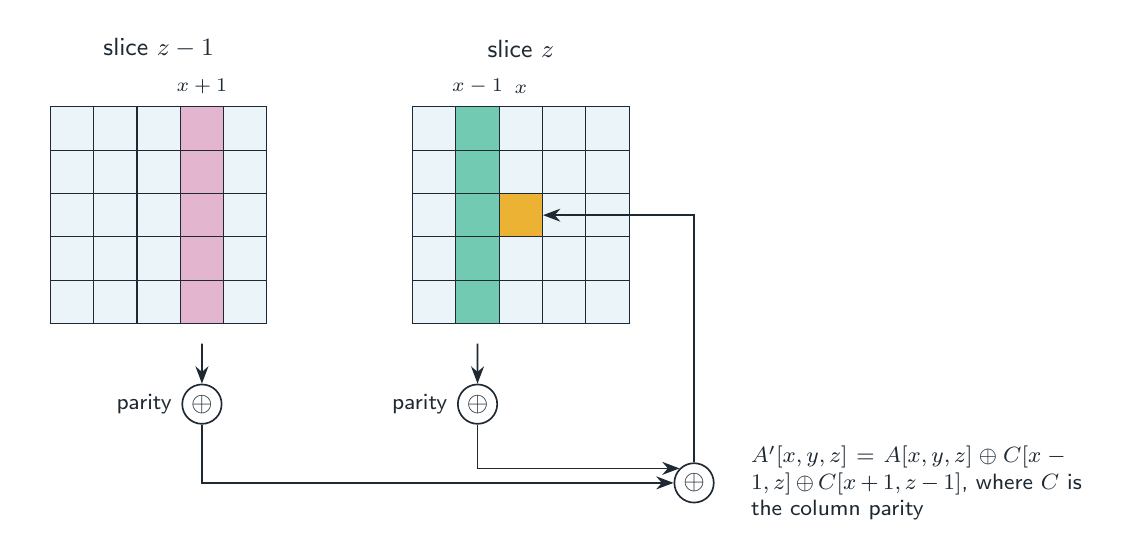
\begin{tikzpicture}[cell/.style={draw=hsink, line width=0.4pt, minimum size=5.5mm, inner sep=0pt}]
  \def\s{0.55}
  % Slice z - 1 (left) and slice z (right).
  \foreach \xx in {0,...,4} \foreach \yy in {0,...,4} {
    \node[cell, fill=hsblue!8] (L\xx\yy) at (\xx*\s, \yy*\s) {};
    \node[cell, fill=hsblue!8] (R\xx\yy) at (4.6+\xx*\s, \yy*\s) {};
  }
  \foreach \yy in {0,...,4} {
    \node[cell, fill=hspurple!55] at (L3\yy) {};
    \node[cell, fill=hsgreen!55] at (R1\yy) {};
  }
  \node[cell, fill=hsorange!80] (T) at (R22) {};
  \node[above=1pt, font=\scriptsize] at (L34.north) {$x+1$};
  \node[above=1pt, font=\scriptsize] at (R14.north) {$x-1$};
  \node[above=1pt, font=\scriptsize] at (R24.north) {$x$};
  \node[above=14pt, font=\sffamily\small] at (L24.north) {slice $z-1$};
  \node[above=14pt, font=\sffamily\small] at (R24.north) {slice $z$};
  % Parities and the XOR.
  \node[add] (p1) at (1.65, -1.3) {$\oplus$};
  \node[add] (p2) at (5.15, -1.3) {$\oplus$};
  \node[add] (sum) at (7.9, -2.3) {$\oplus$};
  \draw[wire] (L30.south) ++(0,-0.25) -- (p1.north);
  \draw[wire] (R10.south) ++(0,-0.25) -- (p2.north);
  \draw[wire] (p1.south) |- (sum.west);
  \draw[wire] (p2.south) |- (sum.north west);
  \node[anchor=east, font=\sffamily\footnotesize] at (p1.west) {parity};
  \node[anchor=east, font=\sffamily\footnotesize] at (p2.west) {parity};
  \draw[wire] (sum.north) |- (T.east);
  \node[anchor=west, font=\sffamily\footnotesize, text width=4.2cm] at (8.5,-2.3)
    {$A'[x,y,z] = A[x,y,z] \oplus C[x-1,z] \oplus C[x+1,z-1]$, where $C$ is the column parity};
  \begin{scope}[on background layer]
    \coordinate (e1) at (12.9, 3.2);
    \node[card, fit=(L00)(R44)(sum)(T)(e1), inner sep=8pt] {};
  \end{scope}
\end{tikzpicture}
\end{document}
